\chapter{Exploratory Data Analysis}

\section{Maximum Likelihood Estimate of a Doubly Stochastic Poisson Process}

Limit order book imbalance is a ratio of limit order volumes between the bid and ask side, and can be calculated for example as $I(t) = \dfrac{V_b(t) - V_a(t)}{V_b(t) + V_a(t)} \in [-1,1]$.
\begin{itemize}
\item We bin the bid/ask volume imbalances in the Limit Order Book into $K$ bins, each being dubbed a ``regime'' of the limit order book. 
\item $Z_t$ is a continuous-time Markov chain that tracks which regime we're in. $Z_t$ takes values in $\{1, \dots , K\}$, and has an infinitesimal generator matrix $G$.
\item Conditional on being in some regime $k$, the arrival of buy and sell market orders follow independent Poisson processes with intensities $\lambda^{\pm}_k$.
\end{itemize}

We have observations of arrivals of buy/sell market orders and of regime switches occurring, all of which are timestamped. Pictorially, a timeline might look like:

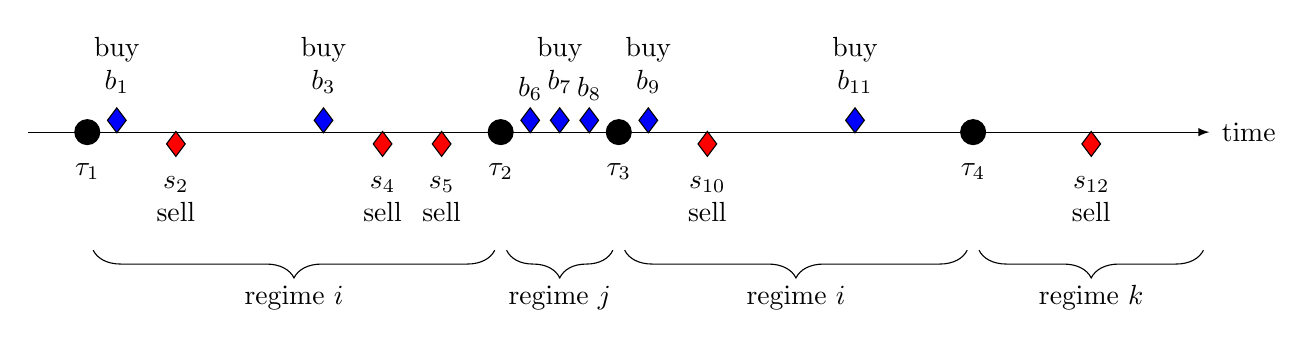
\begin{tikzpicture}[scale=1.5]
	[triangle/.style = {fill=blue!20, regular polygon, regular polygon sides=3 },
	border rotated/.style = {shape border rotate=180}]
	
	
    \draw [>=latex,->] (0,0) -- (10,0) node[draw=none,fill=none,shift=(right:0.5)] {time};
    \draw[mark options={fill=black}, mark size=+3pt] plot[mark=*] coordinates {(.5,0)} node[shift=(down:0.5), align=center] {$\tau_1$};
    \draw[mark options={fill=black}, mark size=+3pt] plot[mark=*] coordinates {(4,0)} node[shift=(down:0.5), align=center] {$\tau_2$};
    \draw[mark options={fill=black}, mark size=+3pt] plot[mark=*] coordinates {(5,0)} node[shift=(down:0.5), align=center] {$\tau_3$};
    \draw[mark options={fill=black}, mark size=+3pt] plot[mark=*] coordinates {(8,0)} node[shift=(down:0.5), align=center] {$\tau_4$};
    
    
	\draw[mark options={fill=blue}, mark size =+3pt, shift=(up:0.1)] plot[mark=diamond*] coordinates {(.75,0)} node[shift=(up:0.7), align=center] {buy \\ $b_1$};
	\draw[mark options={fill=red}, mark size =+3pt, shift=(down:0.1)] plot[mark=diamond*] coordinates {(1.25,0)} node[shift=(down:0.7), align=center] {$s_2$ \\ sell};
	\draw[mark options={fill=blue}, mark size =+3pt, shift=(up:0.1)] plot[mark=diamond*] coordinates {(2.5,0)} node[shift=(up:0.7), align=center] {buy \\ $b_3$};
	\draw[mark options={fill=red}, mark size =+3pt, shift=(down:0.1)] plot[mark=diamond*] coordinates {(3,0)} node[shift=(down:0.7), align=center] {$s_4$ \\ sell};
	\draw[mark options={fill=red}, mark size =+3pt, shift=(down:0.1)] plot[mark=diamond*] coordinates {(3.5,0)} node[shift=(down:0.7), align=center] {$s_5$ \\ sell};

%%% REGIME SWITCH
	
	\draw[mark options={fill=blue}, mark size =+3pt, shift=(up:0.1)] plot[mark=diamond*] coordinates {(4.25,0)} node[shift=(up:0.4), align=center] {$b_6$};
	\draw[mark options={fill=blue}, mark size =+3pt, shift=(up:0.1)] plot[mark=diamond*] coordinates {(4.50,0)} node[shift=(up:0.7), align=center]
{buy \\ $b_7$};
	\draw[mark options={fill=blue}, mark size =+3pt, shift=(up:0.1)] plot[mark=diamond*] coordinates {(4.75,0)} node[shift=(up:0.4), align=center] {$b_8$};
	
%%% REGIME SWITCH

	\draw[mark options={fill=blue}, mark size =+3pt, shift=(up:0.1)] plot[mark=diamond*] coordinates {(5.25,0)} node[shift=(up:0.7), align=center] {buy \\ $b_9$};
	\draw[mark options={fill=red}, mark size =+3pt, shift=(down:0.1)] plot[mark=diamond*] coordinates {(5.75,0)} node[shift=(down:0.7), align=center] {$s_{10}$ \\ sell};
	\draw[mark options={fill=blue}, mark size =+3pt, shift=(up:0.1)] plot[mark=diamond*] coordinates {(7,0)} node[shift=(up:0.7), align=center] {buy \\ $b_{11}$};
	
%%% REGIME SWITCH

	\draw[mark options={fill=red}, mark size =+3pt, shift=(down:0.1)] plot[mark=diamond*] coordinates {(9,0)} node[shift=(down:0.7), align=center] {$s_{12}$ \\ sell};
	
%%% BRACES
	
	\draw [decorate, decoration = {brace, amplitude = 10pt, mirror}]
	(0.55,-1) -- (3.95,-1) node [black, midway, yshift = -0.6cm] {regime $i$};
	\draw [decorate, decoration = {brace, amplitude = 10pt, mirror}]
	(4.05,-1) -- (4.95,-1) node [black, midway, yshift = -0.6cm] {regime $j$}; 
	\draw [decorate, decoration = {brace, amplitude = 10pt, mirror}]
	(5.05,-1) -- (7.95,-1) node [black, midway, yshift = -0.6cm] {regime $i$}; 
	\draw [decorate, decoration = {brace, amplitude = 10pt, mirror}]
	(8.05,-1) -- (9.95,-1) node [black, midway, yshift = -0.6cm] {regime $k$}; 

\end{tikzpicture}

\subsection{Maximum Likelihood Estimation of \texorpdfstring{$G$}{G}}

Let $G$ be the generator matrix for $Z_t$, so $G = \{ q_{ij} \} \in \mathbb{R}^{K \times K}$ where $q_{ij}$ are the transition rates from regime $i$ to regime $j$ for $i\neq j$, and $q_{ii} = - \sum\limits_{j \neq i} q_{ij}$ so that the rows of $G$ sum to 0. 

When $Z_t$ enters regime $i$, the amount of time it spends in regime $i$ is exponentially distributed with rate $v_i = \sum\limits_{j \neq i} q_{ij}$, and when it leaves regime $i$ it will to go regime $j$ with probability $p_{ij} = \dfrac{q_{ij}}{v_i}$. 

From our observations we want to estimate the components of $G$. The holding time in a given regime $i$ is exponentially distributed with pdf $f(t;v_i) = v_i e^{-v_i t}$. For the fictional events in the timeline above, the likelihood function (allowing for repetition of terms) would therefore be:

\begin{align*}
\mathcal{L}(G) &= (v_{i} e^{-v_{i}(\tau_2 - \tau_1)} p_{ij}) (v_{j} e^{-v_{j}(\tau_3 - \tau_2)} p_{ji}) (v_{i} e^{-v_{i}(\tau_4 - \tau_3)} p_{ik}) \dots \\
&= \prod\limits_{i=1}^{K} \prod\limits_{i \neq j} (v_{i}p_{ij})^{N_{ij}(T)} e^{-v_{i}H_i(T)} \\
&= \prod\limits_{i=1}^{K} \prod\limits_{i \neq j} (q_{ij})^{N_{ij}(T)} e^{-v_{i}H_i(T)} \\
\intertext{where:}
N_{ij}(T) & \equiv \mbox{number of transitions from regime $i$ to $j$ up to time $T$} \\
H_{i}(T) & \equiv \mbox{holding time in regime $i$ up to time $T$} \\
\intertext{So that the log-likelihood becomes:} 
\ln \mathcal{L}(G) & = \sum\limits_{i=1}^{K} \sum\limits_{i \neq j} \left[ N_{ij}(T) \ln(q_{ij}) - v_{i} H_i(T) \right] \\
&= \sum\limits_{i=1}^{K} \sum\limits_{i \neq j} \left[ N_{ij}(T) \ln(q_{ij}) - \left( \sum\limits_{i \neq k} q_{ik} H_i(T) \right) \right]
\end{align*}

To get a maximum likelihood estimate $\hat{q}_{ij}$ for transition rates and therefore the matrix $G$, we take the partial derivative of $\ln \mathcal{L}(G)$ and set it equal to zero:

$$\dfrac{\partial \ln \mathcal{L}(G)}{\partial q_{ij}} = \dfrac{N_{ij}(T)}{q_{ij}} - H_i(T) = 0$$
$$ \Rightarrow \hat{q}_{ij} = \dfrac{N_{ij}(T)}{H_i(T)}$$



\subsection{Maximum Likelihood Estimation of \texorpdfstring{$\lambda^{\pm}_k$}{lpmk}}

Now we want to derive an estimate for the intensity of the Poisson process of market order arrivals conditional on being in some regime $k$. We'll look first at just the market buys for some regime $k$. In the above timeline, the market order buy arrival times are indexed by $b_i$. Since we're assuming that the arrival process is Poisson with the same intensity throughout trials, we can consider the inter-arrival time of events conditional on being in regime $k$. Then the MLE derivation follows just as for the CTMC:

\begin{align*}
\mathcal{L}(\lambda^{+}_k ; b_1, \dots, b_N) &= \prod\limits_{i=2}^{N} \lambda^{+}_k e^{-\lambda^{+}_k (b_{i} - b_{i-1})} \\
&= (\lambda^{+}_k)^{N^{+}_k(T)} e^{-\lambda^{+}_k H_k(T)} \\
\intertext{where:}
N^{+}_{k}(T) & \equiv \mbox{number of market order arrivals in regime $k$ up to time $T$} \\
H_{k}(T) & \equiv \mbox{holding time in regime $k$ up to time $T$} \\
\intertext{So that the log-likelihood becomes:} 
\ln \mathcal{L}(\lambda^{+}_k) & = N^{+}_k(T) \ln(\lambda^{+}_k) -\lambda^{+}_k H_k(T)
\intertext{And the ML estimate for $\hat{\lambda}^{+}_k$ is:} 
\dfrac{\partial \ln\mathcal{L} }{\partial \lambda^{+}_k} & = 
\dfrac{N^{+}_k(T)}{\lambda^{+}_k} - H_k(T) = 0
\end{align*}

$$ \Rightarrow \hat{\lambda}^{+}_k = \dfrac{N^{+}_k(T)}{H_k(T)}$$

%Now we want to derive an estimate for the intensity of the Poisson process of market order arrivals conditional on being in some regime $k$. We'll look first at just the market buys for some regime $k$ - call the random variable counting the number of market buys $X$. We want to estimate the intensity, $\lambda^{+}_k$, of the (Poisson) distribution of $X$, which is also the expected value of $X$ as well as its variance. Suppose we have $N$ observations of some fixed time interval of LOB activity in this regime, and the number of market buy events in each trial is $n_i$ for $i=1,\dots,N$.
%
%Assuming the distributions of each trial have the same intensity, the probability mass function gives us that for each $i$:
%
%$$P(X=n_i) = \frac{{\lambda^{+}_k}^{n_i} e^{-\lambda^{+}_k}}{n_i!}$$
%
%Since the trials are independent and identically distributed, the joint density function is:
%
%$$P(n_1, \dots, n_N | \lambda^{+}_k) = P(n_1 | \lambda^{+}_k) \times \dots \times P(n_N | \lambda^{+}_k)$$
%
%So the likelihood function is:
%$$\mathcal{L}(\lambda^{+}_k ; n_1, \dots, n_N) = \prod_{i=1}^{N} P(n_i | \lambda^{+}_k) = \prod_{i=1}^{N} \frac{{\lambda^{+}_k}^{n_i} e^{-\lambda^{+}_k}}{n_i!}$$
%
%Thus the log-likehood can be simplified (using logarithm and exponent identities) as:
%\begin{align*}
%\ln\mathcal{L} &= \ln \left(  \prod_{i=1}^{N} \frac{{\lambda^{+}_k}^{n_i} e^{-\lambda^{+}_k}}{n_i!} \right) \\
%&= \ln \left( \frac{{\lambda^{+}_k}^{\left(\sum_{i=1}^{N} n_i\right)} e^{-N\lambda^{+}_k}}{\prod_{i=1}^{N} n_i!} \right) \\
%&= \ln \left( {\lambda^{+}_k}^{\left(\sum_{i=1}^{N} n_i \right)} \right) - N\lambda^{+}_k - \sum_{i=1}^{N} \ln (n_i !)
%\end{align*}
%
%Now we can get a maximum likelihood estimate for $\lambda^{+}_k$ by taking the partial derivative of $\ln\mathcal{L}$ with respect to $\lambda^{+}_k$ and setting it equal to zero:
%
%$$ \frac{\partial \ln\mathcal{L} }{\partial \lambda^{+}_k} = 
%\dfrac{\sum\limits_{i=1}^{N} n_i}{\lambda^{+}_k} - N = 0$$
%$$\frac{\sum\limits_{i=1}^{N} n_i}{\lambda^{+}_k} = N$$
%$$\lambda^{+}_k = \frac{\sum\limits_{i=1}^{N} n_i}{N}$$

\section{Modeling \texorpdfstring{$I(t)$}{I(t)}: Continuous Time Markov Chain}
Instead of modeling imbalance directly, an alternative approach is to discretize imbalance
into subintervals (called bins), and model a stochastic process that tracks which
bin $I(t)$ falls into. A naive model that can be employed is a continuous-time Markov chain (CTMC).

Let $Z(t)$ be a CTMC taking values in $\left\lbrace 1,\dots , K \right\rbrace$, and having
infinitessimal generator matrix $\mat{G}$.\footnote{Define the terms 
$P_{ij}(t) = P \lbrace Z(t) = j | Z(0) = i \rbrace$. Then the matrices 
$\mat{P}(t) = \lbrace P_{ij}(t) \rbrace$ and $\mat{G}$ satisfy
$\dot{\mat{P}}(t) = \mat{G} \cdot \mat{P}(t)$, and hence $\mat{P}(t) = e^{\mat{G}t}$} 
Conditional on being in some regime $k$, the arrival of buy and sell market orders follow
independent Poisson processes with intensities $\lambda_k^\pm$ (and are hence Markov-modulated
Poisson processes), where $\lambda_k^+$ ($\lambda_k^-$) is the rate of arrivals of market sells (buys).

Given a set of observations of buy/sell market orders and regime switches, we previously derived a
maximum likelihood estimation (MLE) for both the entries of $\mat{G}$ and the values $\lambda_k^\pm$. 
Where $\mat{G} = \lbrace q_{ij} \rbrace \in \mathbb{R}^{K \times K}$, the $q_{ij}$ represent the
transition rates from bin $i$ to $j$ for $i \neq j$, and $q_{ii} = - \sum_{j \neq i} q_ij$ such
that the rows sum to $0$. We found that:
$$ \hat{q}_{ij} = \dfrac{N_{ij}(T)}{H_i(T)} $$
where
\begin{align*} 
N_ij(T) & \equiv \text{number of transitions from bin $i$ to $j$ up to time $T$} \\
H_i(T) & \equiv \text{holding time in bin $i$ up to time $T$}
\end{align*}

Similarly, for the Poisson process intensities $\lambda_k^\pm$, we found:
$$ \hat{\lambda}_k^\pm = \dfrac{N_k^\pm(T)}{H_k(T)} $$
where
\begin{align*} 
N_ij(T) & \equiv \text{number of market orders in bin $k$ up to time $T$} \\
H_i(T) & \equiv \text{holding time in bin $k$ up to time $T$}
\end{align*}

\section{Calibrating a CTMC}
We estimated parameters for a CTMC on a day's worth of LOB data.
Using these parameters, we generated sample paths of the imbalance bins as well as arrival of market orders,
and re-estimated parameters along the sample paths. By doing this for 10,000 paths we obtained histograms for
the parameters (the individual entires of $\mat{G}$ as well as the intensities $\lambda_k^\pm$). 

Using data for \texttt{ORCL} from 2013-05-15, averaging imbalances over a 100ms window, and taking the number
of bins $K=3$, we obtained the following mean values for the parameters:

$$ \mat{G} = \begin{pmatrix} -0.112 & 0.098 & 0.0122 \\
							0.099 & -0.21 & 0.111 \\
							0.0115 & 0.112 & -0.1235 \end{pmatrix}$$
							
$$ \mat{\lambda} = \bordermatrix{  & k=1    & k=2   & k=3   \cr
								+ & 0.121  & 0.081 & 0.048 \cr
								- & 0.0263 & 0.062 & 0.153 } $$			

\section{Next Steps}
\begin{enumerate}
\item Run cross-validation on the old CTMC imbalance model, also varying the averaging time.
\item Check for a unit root in the imbalance time series using the augmented Dickey-Fuller test, after transforming the data using the logit function.
\item Consider a CTMC where the state is actually the pair $(I_{k-1}, I_k)$, with a $k^2 \times k^2$ transition matrix. Cross-validate and compare with regular CTMC.
\end{enumerate}

\section{Cross-validation of CTMC}
To cross-validate the CTMC calibration, the following steps were taken:
\begin{enumerate}
\item An imbalance averaging time (in ms) and number of imbalance bins were fixed. The infinitesimal generator matrix $\mat{G}$ was calculated on the resulting timeseries. 
\item An embedded discrete Markov chain transition matrix $\mat{A}$ was obtained from $\mat{G}$. This effectively says: conditional on a transition from bin $i$, what are the transition probabilities to bin $j$?
\item The stationary distribution, and number ($n$) of steps required to converge to the stationary distribution, was calculated. That is: for $\epsilon > 0$, calculate $n$ such that $||\mat{A}^{n+1} - \mat{A}^n|| < \epsilon$.
\item Find the average number of steps in the timeseries that are required to observe $n$ transitions. This is the size of the timewindow against which to cross-validate. 
\item Remove the cross-validation timewindow (call this the ``removed series'') from the full timeseries (call this the ``remaining series''). Calculate two infinitesimal generator matrices $\mat{G}_{removed}$ and $\mat{G}_{remaining}$.
\item Calculate two error terms for the resulting matrices:
$$err = \sqrt{\dfrac{1}{\#trials} \times \sum\limits_{trials} \left( \dfrac{1}{\#bins^2} \sum\limits_{ij} (\mat{G}_{remaining}(ij) - \mat{G}_{removed}(ij))^2 \right)x} $$
$$\mat{Err} = \sqrt{\dfrac{1}{\#trials} \times \sum\limits_{trials} (\mat{1} - \mat{G}_{removed} \div \mat{G}_{remaining})^2 }$$
where, for $\mat{Err}$, division and squaring are entry-wise and not matrix-wise.
\end{enumerate}

This is following up on the cross-validation results from last time. In those results, in order to obtain the invariant distribution for the Markov chain, we calculated a transition probability matrix $\mat{A}$ for the embedded discrete-time Markov chain and took matrix powers $\mat{A}^n$ until it converged, and then observed the average number of timesteps that it took to see $n$ transitions in the data.

In these results, we instead use the relationship $\dot{\mat{P}} (t) = \mat{P}(t)\mat{G} \; \Rightarrow \; \mat{P}(t) = e^{t\mat{G}}$. Thus we calculate the invariant distribution using the averaging time $\Delta t$ and the number of such timesteps $n$ and observe when $e^{\Delta t\mat{G}n}$ converges. This value $n$ immediately tells us the timewindow size to remove for cross-validation.

\begin{table}[H]
\small
\centering
\caption{New results, convergence threshold 1e-05}
\vspace*{2.5mm}
\begin{tabular}{c|c|c|c|c}
\hline
\bf num bins & & & & \\ averaging time & stationary $n$ & Timewindow size & $err$ & $\mat{Err}$ \\
\hline\hline
3 bins, 100ms & 478 & 47.8s (0.2\% of series) & 0.356402 & 644\% - 11371\% \\
\hline
3 bins, 500ms & 144 & 72s (0.3\% of series) & 0.087631 & 236\% - 985\% \\
\hline
3 bins, 1000ms & 89 & 89s (0.4\% of series) &  0.050605 & 150\% - 480\% \\
\hline
3 bins, 2000ms & 57 & 114s (0.5\% of series) & 0.032076 & 122\% - 725\% \\
\hline
3 bins, 3000ms & 45 & 135s (0.6\% of series) & 0.023662 & 98\% - 552\% \\
\hline
3 bins, 5000ms & 35 & 175s (0.75\% of series) & 0.014182 & 70\% - 514\% \\
\hline
3 bins, 10000ms & 29 & 290s (1.2\% of series) & 0.007361 & 52\% - 496\% \\
\hline
3 bins, 20000ms & 22 & 440s (1.9\% of series) & 0.004447 & 43\% - 1698\% \\
\hline
\hline
5 bins, 100ms & 546 & 54.6s (0.2\% of series) & 0.162690 & 452\% - 6785\% \\
\hline
5 bins, 500ms & 162 & 81s (0.3\% of series) &  0.046204 & 187\% - 2590\% \\
\hline
5 bins, 1000ms & 100 & 100s (0.4\% of series) & 0.029900 & 136\% - 2962\% \\
\hline
5 bins, 2000ms & 65 & 130s (0.6\% of series)  & 0.017340 & 86\% - 2141\% \\
\hline
5 bins, 3000ms & 52 & 156s (0.7\% of series) &  0.012505 & 87\% - Inf\% \\
\hline
5 bins, 5000ms & 42 & 210s (0.9\% of series) & 0.008035 & 66\% - 978\% \\
\hline
5 bins, 10000ms & 31 & 310s (1.3\% of series) & 0.004563 & 45\% - Inf\% \\
\hline
5 bins, 20000ms & 25 & 500s (2.1\% of series) & 0.002485 & 42\% - Inf\% \\
\hline
\end{tabular}
\end{table}

The large errors seen in the error matrix $\mat{Err}$ are attributable to the corner elements: in the case of 3 bins, this would be $G_{13}$ and $G_{31}$. Or, for example, the error matrices for 5 bins at 100ms and at 20000ms looked like:

$$\mat{Err}_{100ms} = \begin{bmatrix}
    6.86 &   8.48 &   5.92 &   9.68 &  11.02\\
    7.57 &   6.82 &   8.80 &  67.58 &   8.31\\
    6.33 &   5.08 &   4.52 &   8.55 &  16.79\\
   14.64 &  54.50 &   8.12 &   6.41 &   7.77\\
    6.82 &  36.76 &   5.47 &   5.86 &   5.04
\end{bmatrix}$$

$$\mat{Err}_{20000ms} = \begin{bmatrix}
    0.79 &   0.99 &   3.63 &  20.23 &    Inf\\
    1.10 &   0.44 &   0.82 &   1.36 &    NaN\\
    2.07 &   0.64 &   0.42 &   0.88 &   3.83\\
    3.64 &   1.66 &   0.85 &   0.57 &   2.81\\
     NaN &    Inf &   1.42 &   1.08 &   0.87
\end{bmatrix}$$

\section{2-dimensional CTMC}
Next we considered a CTMC that tracks not only the imbalance bin, but jointly the imbalance bin and the price change over a subsequent interval. That is to say, the CTMC modelled the joint distribution $(I(t), \Delta S(t))$ where $I(t)$ is the bin corresponding to imbalance averaged over the interval $[t-\Delta t_I, t]$, and $\Delta S(t) = \sgn(S(t+\Delta t_S)-S(t))$, considered individually for the best bid and best ask prices. For 3 bins, this was encoded into one dimension $Z(t)$ as follows:

\begin{table}[H]
\small
\centering
\vspace*{2.5mm}
\begin{tabular}{c|c|c}
\hline
$Z(t)$ & Bin $I(t)$ & $\Delta S(t)$ \\
\hline\hline
1 & Bin 1 & $<0$ \\
\hline
2 & Bin 2 & $<0$ \\
\hline
3 & Bin 3 & $<0$ \\
\hline
4 & Bin 1 & $0$ \\
\hline
5 & Bin 2 & $0$ \\
\hline
6 & Bin 3 & $0$ \\
\hline
7 & Bin 1 & $>0$ \\
\hline
8 & Bin 2 & $>0$ \\
\hline
9 & Bin 3 & $>0$ \\
\hline
\end{tabular}
\end{table}

Here bid and ask prices were considered separately rather than considering the change in mid price. Calibrating a CTMC on the two resulting timeseries $Z_{bid}(t)$ and $Z_{ask}(t)$ yielded some interesting results:


imbalance $\Delta t_I$: 1000ms, price $\Delta t_S$: 500ms

$$\mat{G}_{Z_{bid}} =
\begin{bmatrix}
-0.9928 &   0.0217   &      0 &   0.2826  &  0.5870  &  0.0870  &       0   & 0.0145     &    0 \\

    0.0118  & -0.9647   &     0  &  0.1412 &   0.5882 &   0.2000   &      0   & 0.0118  &  0.0118 \\
         0  &  0.0909  & -1.0000   &      0  &  0.3636  &  0.5455  &       0     & 0  &       0 \\
    0.0146  &  0.0005     &    0  & -0.0792  &  0.0562   & 0.0034 &   0.0036   & 0.0006  &  0.0003 \\
    0.0016 &   0.0052   & 0.0003 &   0.0435  & -0.0897 &   0.0300  &       0   & 0.0080 &   0.0011 \\
    0.0003&    0.0025 &   0.0022  &  0.0053   & 0.0919  & -0.1277     &    0   & 0.0017 &   0.0237 \\
         0  &  0.0345   &      0  &  0.4138  &  0.4138  &  0.1034 &  -1.0000   & 0.0345    &     0 \\
    0.0179   & 0.0179    &     0   & 0.2232   & 0.5536  &  0.1250 &   0.0089  & -0.9732 &   0.0268 \\
    0.0094&    0.0189   &      0  &  0.1132&    0.5189 &  0.3113    &     0   & 0.0094 &  -0.9811
\end{bmatrix}$$


$$\mat{G}_{Z_{ask}} =
\begin{bmatrix}
 -0.9915 &  0.0169 &  0 &  0.2881 &  0.5678 &  0.1017 &   0 &  0.0169 &  0 \\
 0.0106 & -0.9681 &  0 &  0.1277 &  0.5638 &  0.2340 &   0 &  0.0213 &  0.0106 \\
 0  &  0.0588 & -1.0000 &  0 &  0.2941 &  0.5882 &   0 &  0 &  0.0588 \\
 0.0121 &  0.0005 &  0 & -0.0775 &  0.0580 &  0.0034 &  0.0027 &  0.0005 &  0.0003 \\
 0.0016 &  0.0058 &  0.0002 &  0.0448 & -0.0898 &  0.0297 &   0 &  0.0065 &  0.0011 \\
 0.0003 &  0.0025 &  0.0039 &  0.0059 &  0.0907 & -0.1311 &   0 &  0.0008 &  0.0270 \\
 0 &  0.0476 &  0 &  0.1905 &  0.5714 &  0.1429 & -1.0000 &  0.0476 &   0 \\
 0 &  0.0440 &  0 &  0.1319 &  0.6374 &  0.1429 &   0 & -0.9890 &  0.0330 \\
 0.0085 &  0.0254 &  0.0085 &  0.0847 &  0.5169 &  0.3220 &   0 &  0.0169 & -0.9831

\end{bmatrix}$$

Using these matrices, we can compute conditional probabilities. For example, we can ask: conditional on being in bin 1 (more bid volume than ask) and on the bid price changing, what is the probability that the change will be greater than 0? less than 0?

Again, converting the generator matrix to the embedded discrete time Markov chain matrix proves enlightening for these calculations:

$$\mat{A}_{Z_{bid}} = 
\begin{bmatrix}
         0  &  0.0219 &        0 &   0.2847 &   0.5912 &   0.0876 &        0 &   0.0146 &        0\\
    0.0122  &       0 &        0 &   0.1463 &   0.6098 &   0.2073 &        0 &   0.0122 &   0.0122\\
         0  &  0.0909 &        0 &        0 &   0.3636 &   0.5455 &        0 &        0 &        0\\
    0.1839  &  0.0065 &        0 &        0 &   0.7097 &   0.0435 &   0.0452 &   0.0081 &   0.0032\\
    0.0174  &  0.0581 &   0.0029 &   0.4855 &        0 &   0.3343 &        0 &   0.0891 &   0.0126\\
    0.0022  &  0.0197 &   0.0175 &   0.0416 &   0.7199 &        0 &        0 &   0.0131 &   0.1860\\
         0  &  0.0345 &        0 &   0.4138 &   0.4138 &   0.1034 &        0 &   0.0345 &        0\\
    0.0183  &  0.0183 &        0 &   0.2294 &   0.5688 &   0.1284 &   0.0092 &        0 &   0.0275\\
    0.0096  &  0.0192 &        0 &   0.1154 &   0.5288 &   0.3173 &        0 &   0.0096 &        0
\end{bmatrix}$$

Generator matrices $\mat{G}_{bid}$ and $\mat{G}_{ask}$ were estimated for the resulting timeseries. These were converted to one-step probability matrices $\mat{P}_{bid}$ and $\mat{P}_{ask}$ using the formula $\mat{P} = e{\mat{G}\Delta t}$, where $\Delta t$ is the imbalance averaging period. What this matrix encodes are the conditional one-step transition probabilities - for each entry $\mat{P}_{ij}$ we have:
\begin{align*}
\mat{P}_{ij} & = \mathbb{P} \left[Z_n \in j \; | \; Z_{n-1} \in i \right] \\
&= \mathbb{P}\left[(\rho_n, \Delta S_n) \in j \; | \; (\rho_{n-1}, \Delta S_{n-1}) \in i \right]
\end{align*}

The aim is to use these $\mat{P}$ matrices to compute conditional probabilities of price changes. For example, we can ask: if we are currently in imbalance bin 1, and previous were also in bin 1 and saw a negative price change, what is the probability of again seeing a negative price change?

Since each state $(\rho_n, \Delta S_n) \in j$ is actually comprised of two states, say $\rho_n \in k, \Delta S_n \in m$, we can re-write these entries of $\mat{P}$ as being:
\begin{align*}
& \mathbb{P}\left[ \rho_n \in i, \Delta S_n \in j \; | \; \rho_{n-1} \in k, \Delta S_{n-1} \in m \right] \\
=\;  & \mathbb{P}\left[ \rho_n \in i, \Delta S_n \in j \; | \; B \right]
\end{align*}
where we're using the shorthand $B = (\rho_{n-1} \in k, \Delta S_{n-1} \in m)$ to represent the states in the previous timestep. Using Bayes' Rule, we can write:
$$ \mathbb{P}\left[ \Delta S_n \in j \; | \; B, \rho_n \in i \right] = \dfrac{\mathbb{P}\left[ \rho_n \in i, \Delta S_n \in j \; | \; B \right]}{\mathbb{P}\left[ \rho_n \in i \; | \; B \right]} $$
The left-hand-side value is exactly the conditional probability in price change that we're interested in finding, the numerator is each individual entry of the one-step probability matrix $\mat{P}$, and the denominator can be computed as:
$$\mathbb{P}\left[ \rho_n \in i \; | \; B \right] = \sum\limits_j \mathbb{P}\left[ \rho_n \in i,  \Delta S_n \in j \; | \; B \right]$$

Using 3 bins, 1000ms imbalance averaging, and 500ms price change, we computed $\mat{P}_{bid}$:

$$  \begin{smallmatrix}
    \Delta S_n < 0 \rightarrow \\
    \Delta S_n = 0 \rightarrow \\
    \Delta S_n > 0 \rightarrow
  \end{smallmatrix}
  \left [
    \begin{smallmatrix}
\overmat{\rho_n = 1}{.67 & .05 & .04 & .01 & .03 & .04 & .00 & .05 & .05} & \overmat{\rho_n = 2}{.02 & .50 & .12 & .01 & .00 & .02 & .05 & .01 & .02} & 
\overmat{\rho_n = 3}{.00 & .00 & .52 & .00 & .01 & .00 & .00 & .00 & .00} \\
.33 & .95 & .96 & .99 & .97 & .96 & .41 & .93 & .95 & .96 & .49 & .87 & .98 & .99 & .97 & .91 & .48 & .96 & .98 & .95 & .47 & .95 & .96 & .93 & .98 & .88 & .34 \\ \undermat{\Delta S_{n-1} < 0}{.00 & .00 & .00} & 
\undermat{}{.00 & .00 & .00} & 
\undermat{\Delta S_{n-1} > 0}{.58 & .02 & .00} & 
\undermat{}{.02 & .01 & .00} & 
\undermat{\Delta S_{n-1} = 0}{.01 & .01 & .01} & 
\undermat{}{.05 & .51 & .01} & 
\undermat{}{.02 & .04 & .01} & 
\undermat{}{.05 & .03 & .02} & 
\undermat{}{.02 & .12 & .66}
    \end{smallmatrix}
  \right ]
$$

\section{In-Sample Backtesting of Naive Trading Strategies}
As a refresher: 

We are a considering a CTMC for the joint distribution $(I(t), \Delta S(t))$ where $I(t) \in \lbrace 1,2,\dots,\#_{bins} \rbrace$ is the bin corresponding to imbalance averaged over the interval $[t-\Delta t_I, t]$, and $\Delta S(t) = \text{sign}(S(t+\Delta t_S)-S(t)) \in \lbrace -1, 0, 1 \rbrace$, considered individually for the best bid and best ask prices. The pair $(I(t), \Delta S(t))$ was then reduced into one dimension with a simple encoding.

From the resulting timeseries we estimated a generator matrix $\mat{G}$ and used it to obtain a one-step transition probability matrix $\mat{P} = e^{\mat{G}\Delta t_I}$. The entries of $\mat{P}$ contain the conditional probabilities $\mathbb{P}\left[ \rho_{curr}, \Delta S_{curr} \; | \; \rho_{prev}, \Delta S_{prev} \right]$, from which we can solve for the probability of now seeing a given price change ($\Delta S_{curr}$) conditional on the current imbalance, the previous imbalance, and the previous price change.

For example, one such conditional probability matrix $\mat{P_C}$ (using 3 imbalance bins) was:

$$  \begin{smallmatrix}
    \Delta S_n < 0 \rightarrow \\
    \Delta S_n = 0 \rightarrow \\
    \Delta S_n > 0 \rightarrow
  \end{smallmatrix}
  \left [
    \begin{smallmatrix}
\overmat{\rho_n = 1}{.67 & .05 & .04 & .01 & .03 & .04 & .00 & .05 & .05} & \overmat{\rho_n = 2}{.02 & .50 & .12 & .01 & .00 & .02 & .05 & .01 & .02} & 
\overmat{\rho_n = 3}{.00 & .00 & .52 & .00 & .01 & .00 & .00 & .00 & .00} \\
.33 & .95 & .96 & .99 & .97 & .96 & .41 & .93 & .95 & .96 & .49 & .87 & .98 & .99 & .97 & .91 & .48 & .96 & .98 & .95 & .47 & .95 & .96 & .93 & .98 & .88 & .34 \\ \undermat{\Delta S_{n-1} < 0}{.00 & .00 & .00} & 
\undermat{}{.00 & .00 & .00} & 
\undermat{\Delta S_{n-1} > 0}{.58 & .02 & .00} & 
\undermat{}{.02 & .01 & .00} & 
\undermat{\Delta S_{n-1} = 0}{.01 & .01 & .01} & 
\undermat{}{.05 & .51 & .01} & 
\undermat{}{.02 & .04 & .01} & 
\undermat{}{.05 & .03 & .02} & 
\undermat{}{.02 & .12 & .66}
    \end{smallmatrix}
  \right ]
$$

\vspace{0.5cm}
Immediately evident from $\mat{P_C}$ is that in most cases we are expecting no price change. In fact, the only cases in which the probability of a price change is $>0.5$ show evidence of \textit{momentum}; for example, the way to interpret the value in row 1, column 1 is: if $\rho_{prev} = \rho_{curr} = 1$ and previously we saw a downward price change, then we expect to again see a downward price change. In fact, the best way to summarize the matrix is:

$$ \mathbb{P} \left[ \Delta S_{curr} = \Delta S_{prev} \; | \; \rho_{prev} = \rho_{curr} \right] > 0.5 $$

\begin{algorithm}
\caption{Naive Trading Strategy}
\begin{algorithmic}[1]
\State $cash = 0$
\State $asset = 0$
\For{$t=2 \; : \; \texttt{length}(timeseries)$}
	\If {$\mathbb{P} \left[ \Delta S_{curr} < 0 \; | \; \rho_{curr}, \rho_{prev}, \Delta S_{prev} \right] > 0.5$}
		\State $cash \pluseq data.BuyPrice(\textit{t})$
		\State $asset \mineq 1$
	\ElsIf {$\mathbb{P} \left[ \Delta S_{curr} > 0 \; | \; \rho_{curr}, \rho_{prev}, \Delta S_{prev} \right] > 0.5$}
		\State $cash \mineq data.SellPrice(\textit{t})$	
		\State $asset \pluseq 1$
	\EndIf
\EndFor
\If {$asset > 0$} 
	\State $cash \pluseq asset \times data.BuyPrice(\textit{t})$
\ElsIf {$asset < 0$} 
	\State $cash \pluseq asset \times data.SellPrice(\textit{t})$	
\EndIf
\end{algorithmic}
\end{algorithm}

\begin{algorithm}
\caption{Naive+ Trading Strategy}
\begin{algorithmic}[1]
\State $cash = 0$
\State $asset = 0$
\State $LO_{posted} = \texttt{False}$
\For{$t=2 \; : \; \texttt{length}(timeseries)$}
	\If {$\mathbb{P} \left[ \Delta S_{curr} < 0 \; | \; \rho_{curr}, \rho_{prev}, \Delta S_{prev} \right] > 0.5$}
		\State $cash \pluseq data.BuyPrice(\textit{t})$
		\State $asset \mineq 1$
		\State $LO_{posted} = \texttt{False}$
	\ElsIf {$\mathbb{P} \left[ \Delta S_{curr} > 0 \; | \; \rho_{curr}, \rho_{prev}, \Delta S_{prev} \right] > 0.5$}
		\State $cash \mineq data.SellPrice(\textit{t})$	
		\State $asset \pluseq 1$
		\State $LO_{posted} = \texttt{False}$
	\ElsIf {$\mathbb{P} \left[ \Delta S_{curr} = 0 \; | \; \rho_{curr}, \rho_{prev}, \Delta S_{prev} \right] > 0.5$}
		\State $LO_{posted} = \texttt{True}$
	\EndIf
	\If {$LO_{posted}$}
		\For{$MO \in ArrivedMarketOrders(t,t+1)$}		
			\If {$MO == Sell$}
				\State $cash \mineq data.BuyPrice(\textit{t})$	
				\State $asset \pluseq 1$
			\ElsIf {$MO == Buy$}
				\State $cash \pluseq data.SellPrice(\textit{t})$
				\State $asset \mineq 1$
			\EndIf
		\EndFor
	\EndIf
\EndFor
\If {$asset > 0$} 
\State $cash \pluseq asset \times data.BuyPrice(\textit{t})$
\ElsIf {$asset < 0$} 
\State $cash \pluseq asset \times data.SellPrice(\textit{t})$	
\EndIf
\end{algorithmic}
\end{algorithm}

\begin{algorithm}
\caption{Naive++ Trading Strategy}
\begin{algorithmic}[1]
\State $cash = 0$
\State $asset = 0$
\State $LOBuy_{posted} = \texttt{False}$
\State $LOSell_{posted} = \texttt{False}$
\For{$t=2 \; : \; \texttt{length}(timeseries)$}
	\If {$\mathbb{P} \left[ \Delta S_{curr} < 0 \; | \; \rho_{curr}, \rho_{prev}, \Delta S_{prev} \right] > 0.5$}
		\State $LOBuy_{posted} = \texttt{False}$
		\State $LOSell_{posted} = \texttt{True}$
	\ElsIf {$\mathbb{P} \left[ \Delta S_{curr} > 0 \; | \; \rho_{curr}, \rho_{prev}, \Delta S_{prev} \right] > 0.5$}
		\State $LOBuy_{posted} = \texttt{True}$
		\State $LOSell_{posted} = \texttt{False}$
	\ElsIf {$\mathbb{P} \left[ \Delta S_{curr} = 0 \; | \; \rho_{curr}, \rho_{prev}, \Delta S_{prev} \right] > 0.5$}
		\State $LOBuy_{posted} = \texttt{False}$
		\State $LOSell_{posted} = \texttt{False}$
	\EndIf

	\For{$MO \in ArrivedMarketOrders(t,t+1)$}		
		\If {$MO == Sell \; \land \; LOBuy_{posted}$}
			\State $cash \mineq data.BuyPrice(\textit{t})$	
			\State $asset \pluseq 1$
		\ElsIf {$MO == Buy \; \land \; LOSell_{posted}$}
			\State $cash \pluseq data.SellPrice(\textit{t})$
			\State $asset \mineq 1$
		\EndIf
	\EndFor
\EndFor
\If {$asset > 0$} 
\State $cash \pluseq asset \times data.BuyPrice(\textit{t})$
\ElsIf {$asset < 0$} 
\State $cash \pluseq asset \times data.SellPrice(\textit{t})$	
\EndIf
\end{algorithmic}
\end{algorithm}

We backtested a number of naive trading strategies, outlined here, based on this key observation. In plain terms, the Naive trading strategies can be interpreted as follows:

\paragraph{Naive Trading Strategy}  Using the conditional probabilities obtained from $\mat{P_C}$, we will execute a buy (resp. sell) market order if the probability of an upward (resp. downward) price change is $> 0.5$.

\paragraph{Naive+ Trading Strategy} Extending the naive trading strategy, if we anticipate no change then we'll additionally keep limited orders posted at the touch, front of the queue. We'll track MO arrival, assume we always get excuted, and immediately repost the limit orders.

\paragraph{Naive++ Trading Strategy} We won't execute market orders or keep limit orders at the touch. Using the conditional probabilities obtained from $\mat{P_C}$, if we expect a downward (resp. upward) price change then we'll add a limit order to the sell (resp. buy) side, and hopefully pick up an agent who is executing a market order going against the price change momentum. 

\paragraph{Naive- Trading Strategy} We additionally considered a trading strategy, for benchmark purposes, which used only current imbalance to predict future price change. But actually this predicted $\mathbb{P} \left[ \Delta S_{curr} = 0 \right] > 0.5$ at all times, so we could not run a strategy off it.

Backtesting these trading strategies required a choice of parameters for $\Delta t_S$, the price change observation period, $\Delta t_I$, the imbalance averaging period, and $\#_{bins}$, the number of imbalance bins. Through a brute force calibration technique we found that $\#_{bins} = 4$ provided the highest expected number of successful trades for most tickers, so this was chosen as a constant. Similarly, we empirically saw that calibration always yielded $\Delta t_S = \Delta t_I$, so this was taken as a given. Then each backtest consisted of first calibrating the value $\Delta t_I$ from one day of data by maximizing the intra-day Sharpe ratio, then using the calibrated parameters to backtest the entire year.

\begin{figure}
  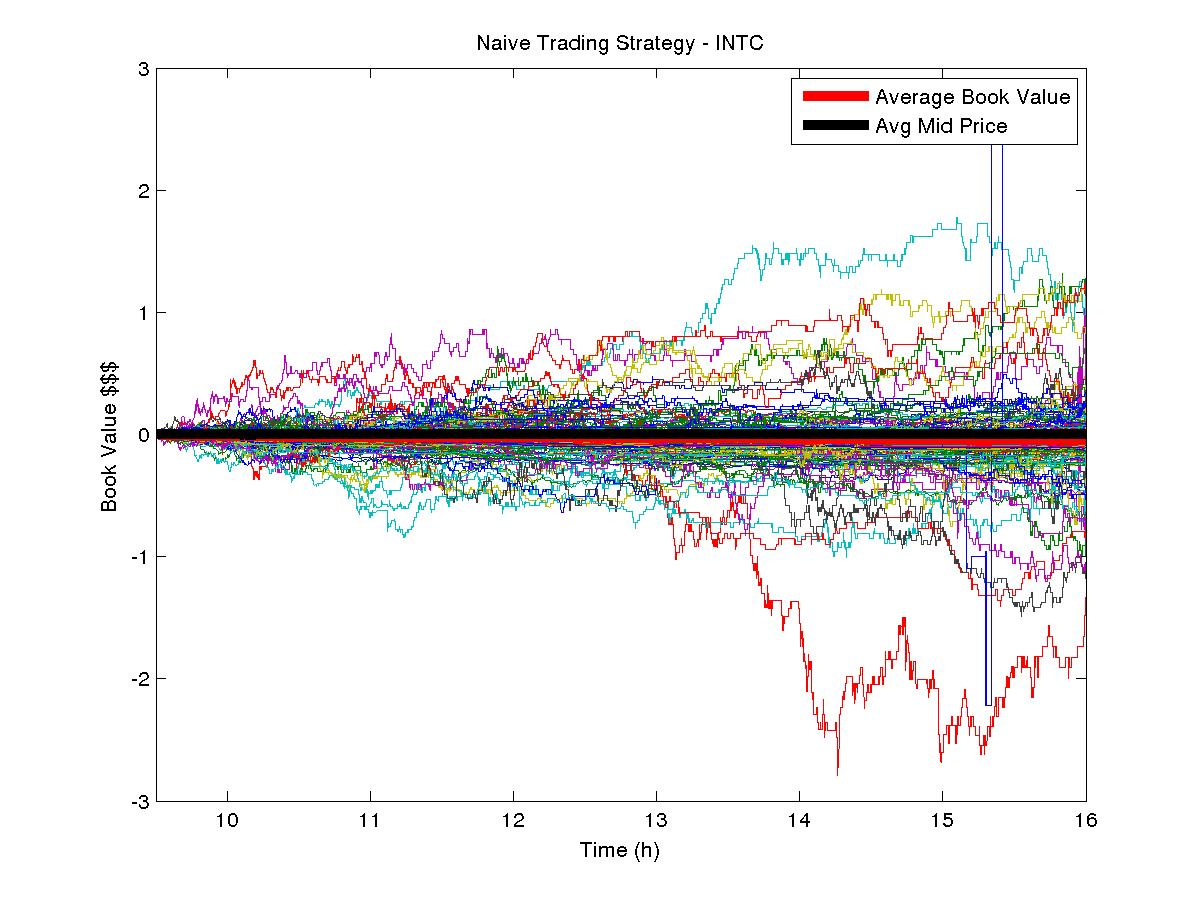
\includegraphics[width=\textwidth]{Figs/fig-INTC-year-bookvals}
  \caption{INTC: Bookvalue against time of trading day.}
\end{figure}

\begin{figure}
  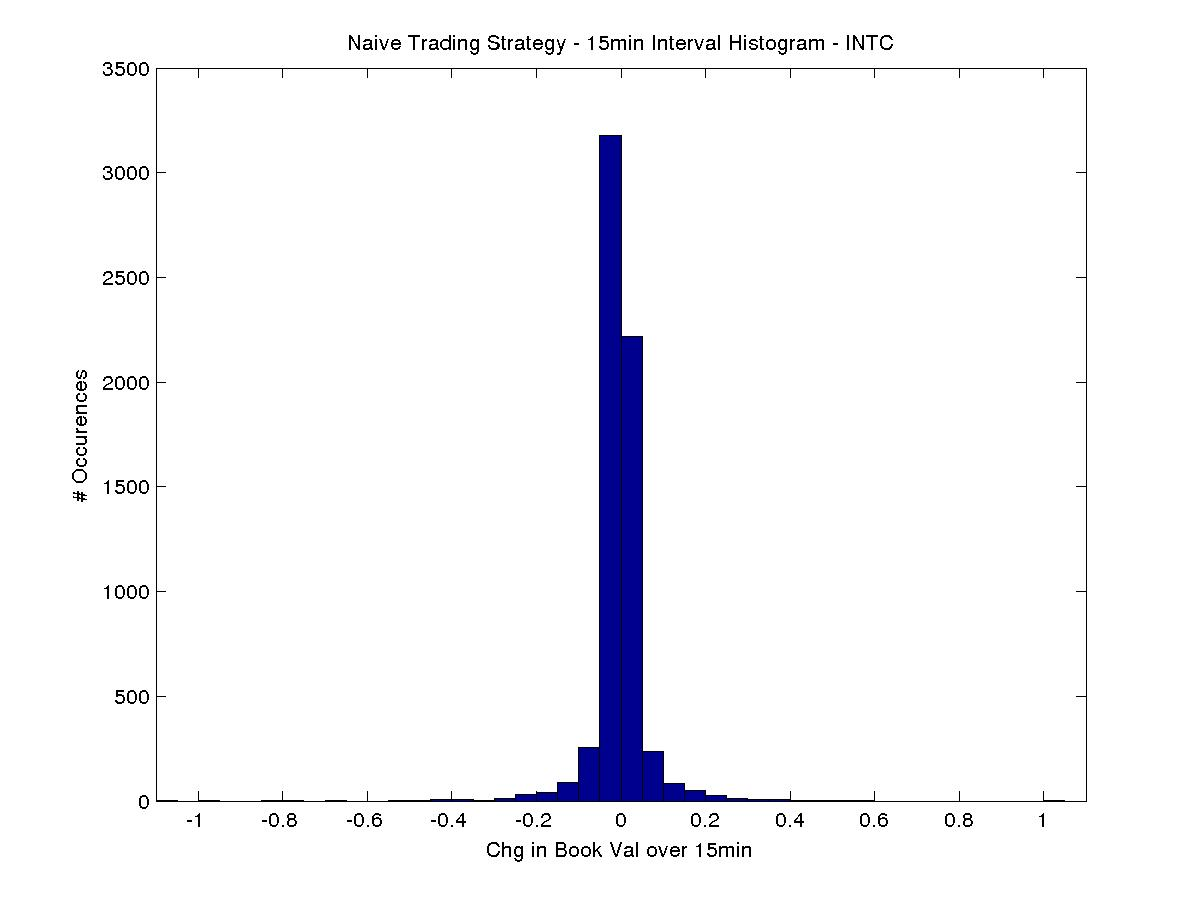
\includegraphics[width=\textwidth]{Figs/fig-INTC-15min-hist}
  \caption{INTC: Histogram of 15min bookvalue changes.}
\end{figure}

\begin{figure}[h]
  \centering
  \begin{tabular}{cc}
  	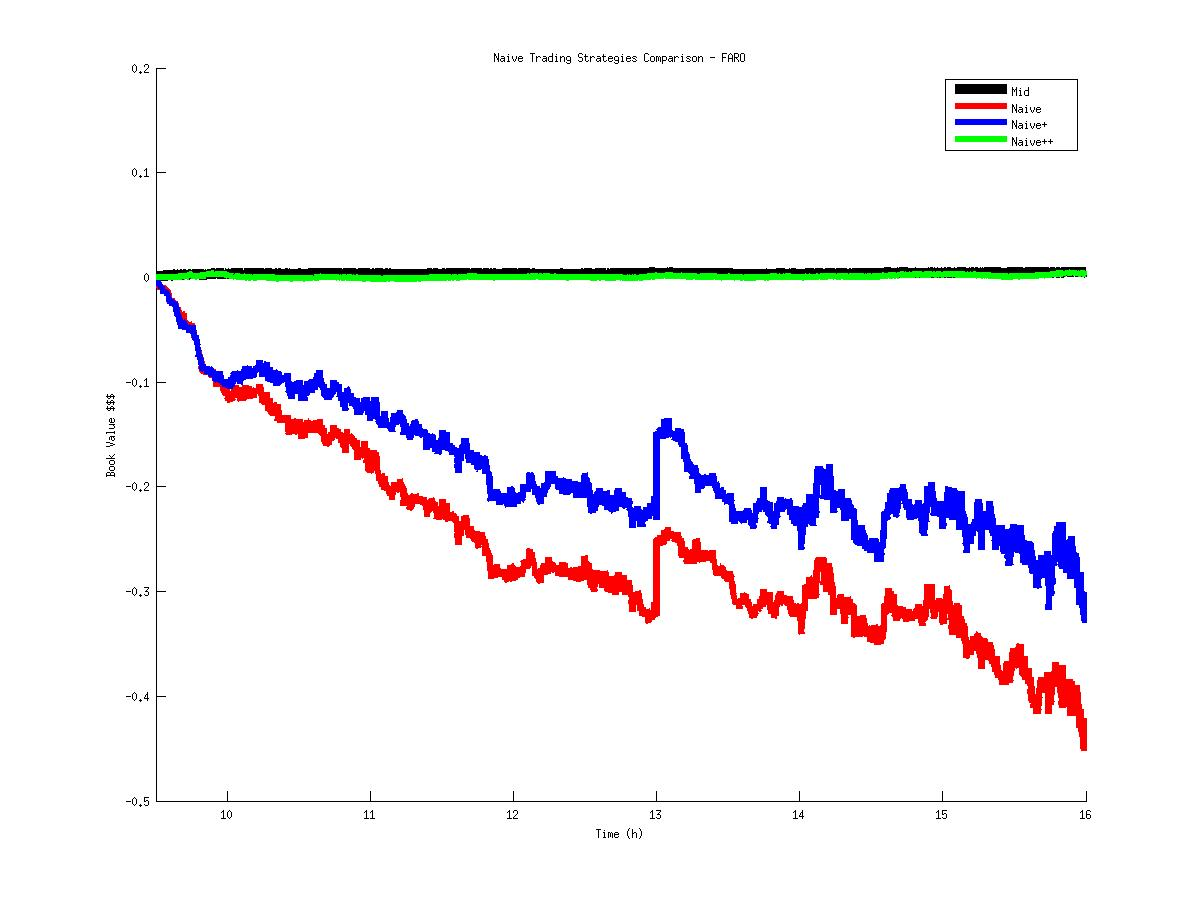
\includegraphics[width=0.45\textwidth]{Figs/fig-compare-strat-FARO} & 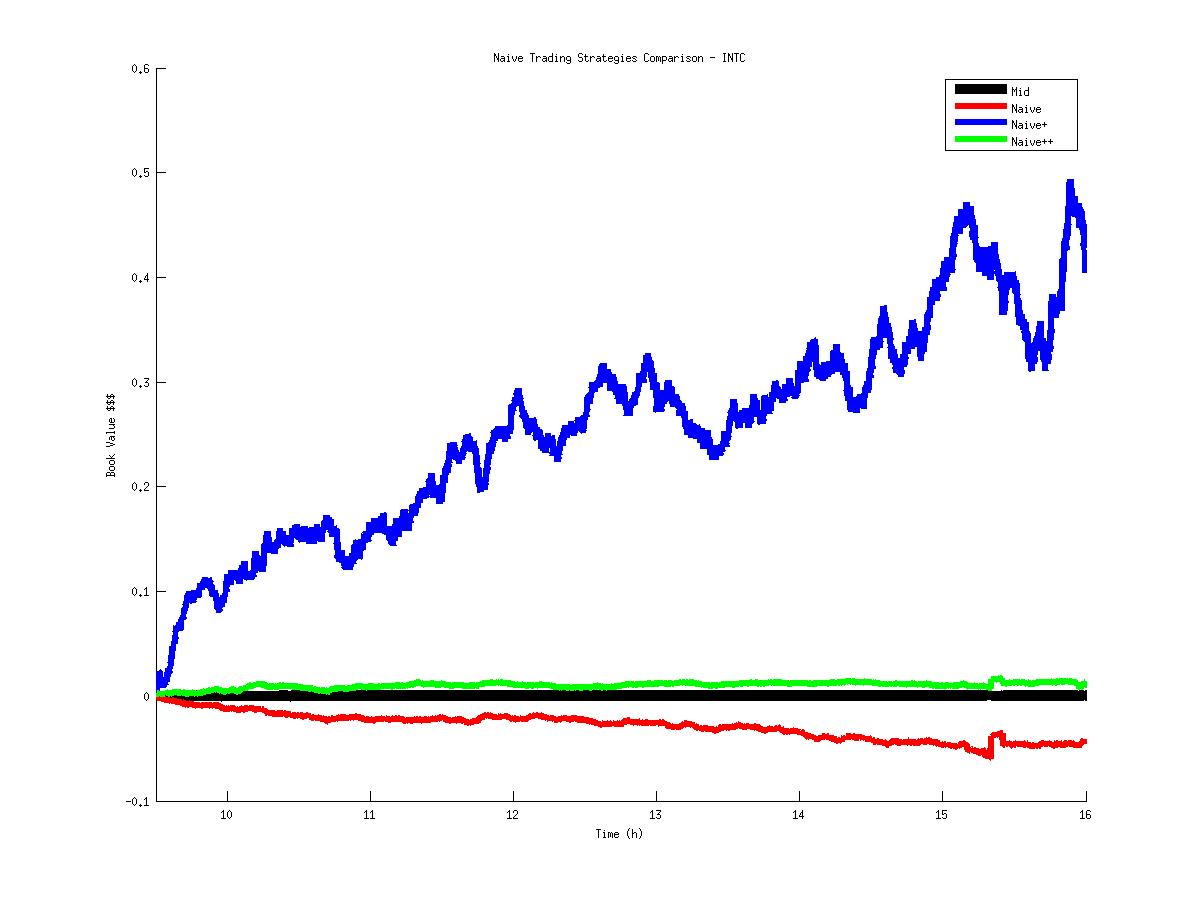
\includegraphics[width=0.45\textwidth]{Figs/fig-compare-strat-INTC} \\
  	FARO & INTC \\
  	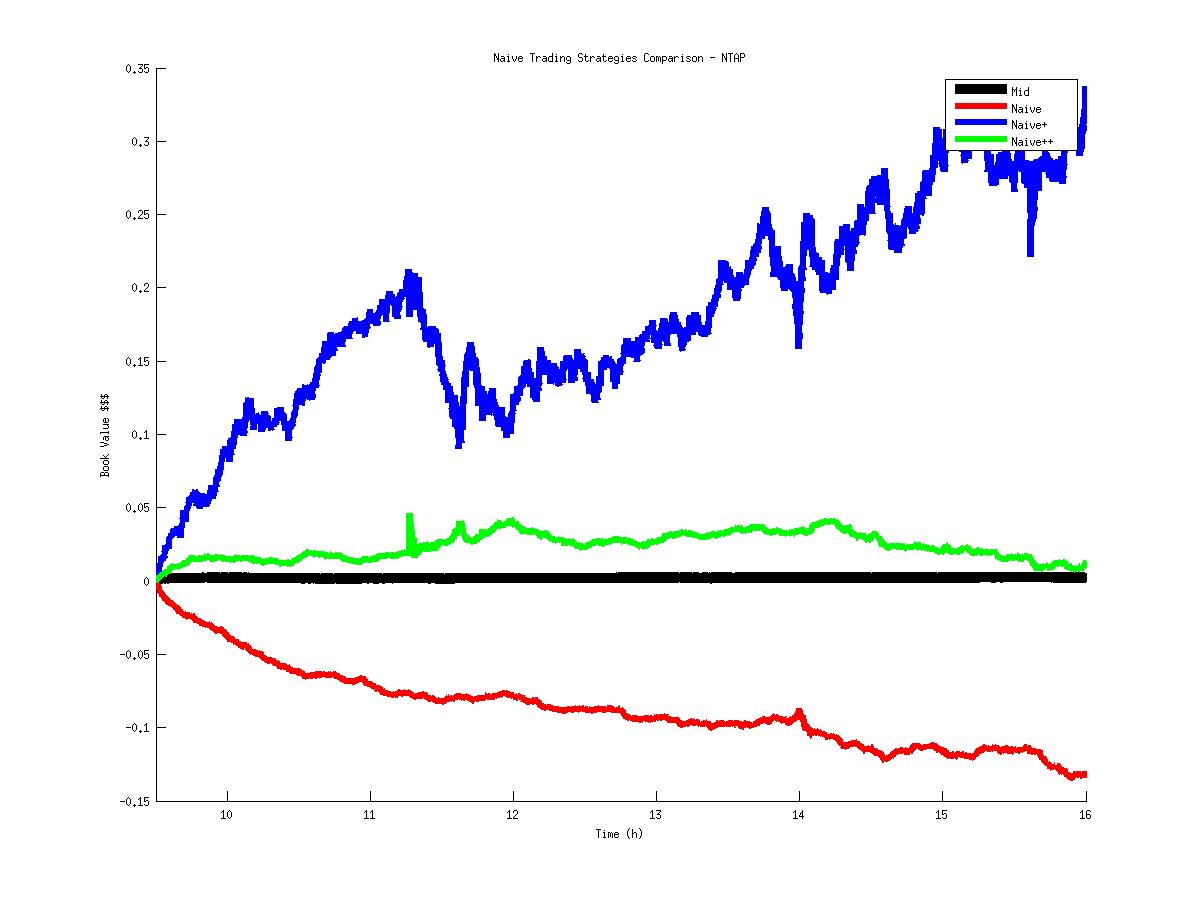
\includegraphics[width=0.45\textwidth]{Figs/fig-compare-strat-NTAP} & 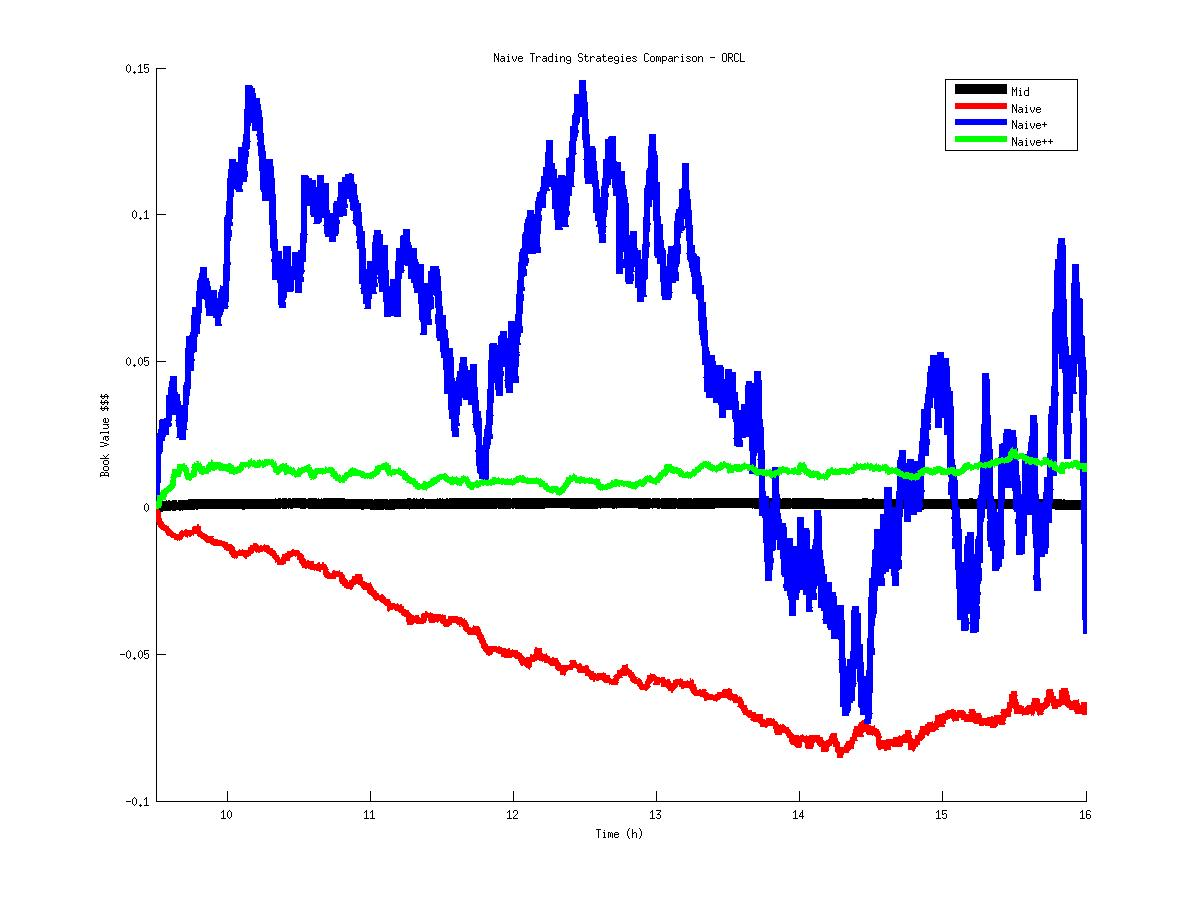
\includegraphics[width=0.45\textwidth]{Figs/fig-compare-strat-ORCL} \\
  	  	NTAP & ORCL \\
    \multicolumn{2}{c}{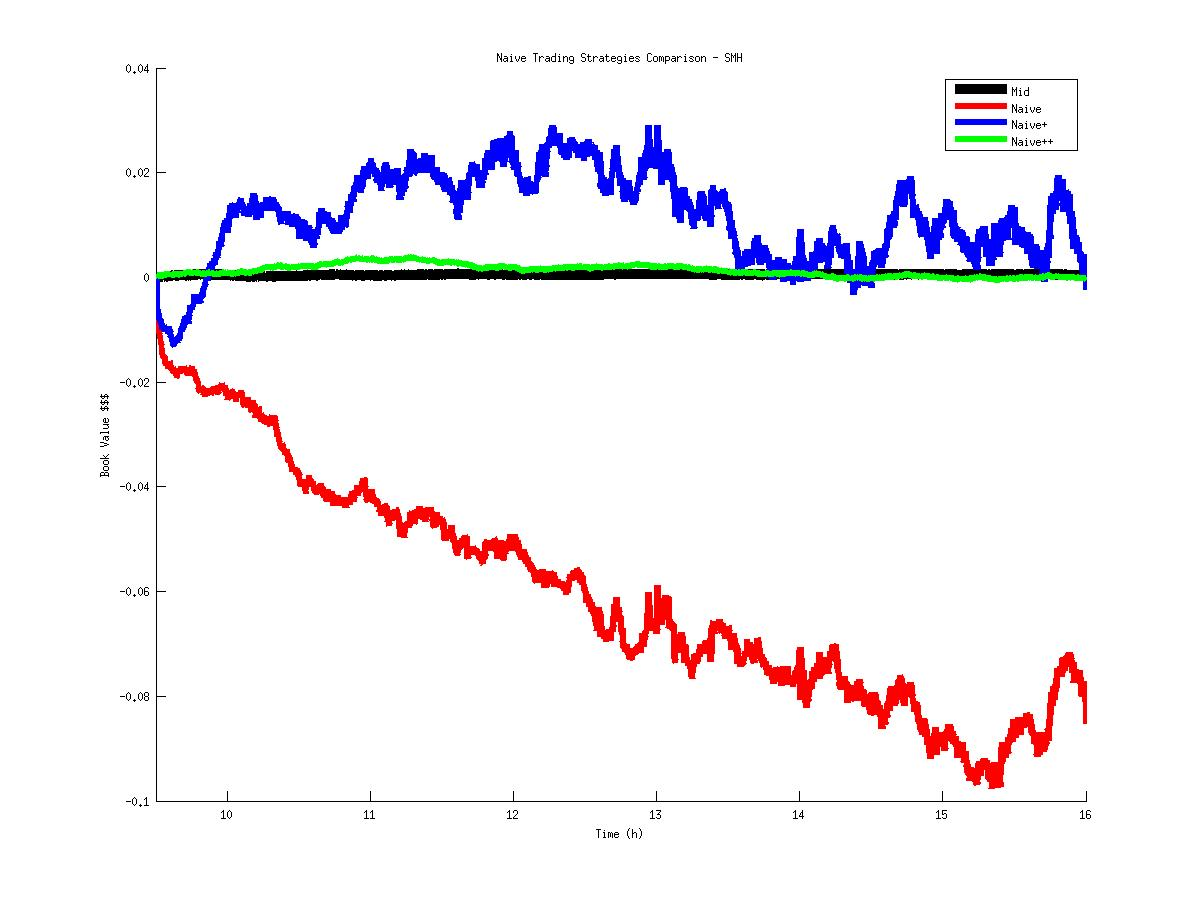
\includegraphics[width=0.45\textwidth]{Figs/fig-compare-strat-SMH} }\\
    \multicolumn{2}{c}{SMH}  	
  \end{tabular}
  \caption{Comparison of Naive (red), Naive+ (blue), and Naive++ (green) trading strategies, with benchmark Midprice (black). Plotted are bookvalues against time of trading day, averaged across trading year.}
  \label{fig:comp}
\end{figure}

\section{Conclusions from Naive Trading Strategies}

To properly compare the Naive trading strategies, it must be understood that the Naive+ strategy has the Naive built into it - thus it's actually the difference between the two that needs to be assessed to ascertain the effect of posting Limit Orders when no price change is predicted. As seen in Figure \ref{fig:comp}, the Naive trading strategy on average underperformed the average mid price, while the Naive+ (adding at-the-touch limit orders when no change was predicted) and Naive++ (adding limit orders to adversely selecting agents that traded against the price change momentum) strategies both on average generated revenue. 

\paragraph{Question 1} Why is the Naive strategy producing, on average, normalized losses? Especially so when considering that we are \underline{in-sample backtesting}. On calibration, we see that our intra-day sharpe ratio is around 0.01 or 0.02 when we choose our optimal parameters, so at the very least on the calibration date the strategy produces positive returns. The remainder of the calendar days are out-of-sample, as the parameters are (likely) not optimal. This suggests non-stationary data, and in particular not every day can be modelled by the same Markov chain. The problem may be exaggerated by the fact that we're calibrating on the first trading day of the calendar year, when we might expect reduced, or at least non-representative, trading activity. Further, we're currently obtaining the $\mat{P_C}$ probability matrix using only bid-side data, not sell-side or mid, and we're ignoring the bid-ask spread. Thus predicting a ``price change'' may be insufficient when considering a monetizable opportunity, as we won't be able to profit off a predicted increase followed by a predicted decrease unless the interim mid-price move is greater than the bid-ask spread (assuming constant spread). This suggests a potential straightforward modification to the strategy.

\paragraph{Question 2} Why do the Naive+ and ++ strategies outperform the Naive strategy? This is particularly interesting since the probabilities are being obtained from the same matrix. The obvious difference between the successful and nonsuccessful strategies is that the former (a) uses limit orders, and (b) executes when we predict a zero change, whereas the latter uses (a) market orders, and (b) executes when we do predict nonzero change.

(a) obviously leads to a different transaction price being used: if I buy with a LO I'm paying the bid price, whereas buying with a MO I pay the ask price. If I value the stock using the mid price, and the mid price doesn't move as a result of my transaction, then with LO I'm buying the asset for less than I'm valuing it at, and with MO I'm paying more than its value.

(b) seems to be the largest flaw in the Naive strategy, to which there are two factors. One, we are not predicting the magnitude of the price change, only whether it is zero or nonzero. Two, from the probabilities presented above, \textit{we will only predict a price change if we've already seen a price change}. Thus we're effectively reacting too late. 

Here's how this works adversely. Suppose a stock has bid/ask quotes of \$9.99/\$10.01, for a bid-ask spread of \$0.02 and a mid of \$10.

\begin{enumerate}
\item Imbalance = 1 (pressure for upward price move). [$NPV = 0$]
\item Bid/ask goes up to \$10.00/\$10.02. [$NPV = 0$]
\item Imbalance = 1. We predict another $>0$ price change. [$NPV = 0$]
\item We buy 1 share (at \$10.02). [$NPV = -0.01$]
\item Bid/ask goes up to \$10.01/\$10.03. [$NPV = 0$]
\item Imbalance = -1 (pressure for a downward move). [$NPV = 0$]
\item Bid/ask goes down to \$10.00/\$10.02. [$NPV = -0.01$]
\item Imbalance = -1. We predict another $<0$ price change. 
\item We sell 1 share (at \$10.00). [$NPV = -0.02$]
\item Bid/ask goes down to \$9.99/\$10.01. [$NPV = -0.02$]
\end{enumerate}

In this example the price goes up and back down by two cents to return to where it started, and in the process we lost \$0.02. Now imagine what happens if we price goes up by one cent, up by one cent, then down by ten cents, down by one cent. In this case we lose \$0.11. We're unable to predict that initial upward or downward price change, and only react to it. 

\paragraph{Ideas to Explore and Next Steps}
\begin{itemize}
\item Model the mid price instead of the bid or ask, hold the bid-ask spread as a constant (average observed), and predict price changes at least as great as the spread, instead of simply non-zero.
\item Calculate imbalance using a weighted average of the best $n$ bid (resp. ask) prices. This may reduce noise in the signal, have an effect on the size of the imbalance averaging window, and be a stronger predictor.
\item Transition to exploring the stochastic control problem.
\end{itemize}
